\documentclass[aspectratio=169,11pt]{beamer}

% ── Packages ──────────────────────────────────────────────────────────────────
\usepackage{graphicx}
\usepackage{booktabs}
\usepackage{array}
\usepackage[T1]{fontenc}
\usepackage{lmodern}
\usepackage{xcolor}
\usepackage{tikz}
\usetikzlibrary{calc, positioning}
\usepackage{amsmath}
\usepackage{hyperref}
\usepackage{siunitx}
\usepackage{colortbl}

% ── Colour Palette ────────────────────────────────────────────────────────────
\definecolor{DeepNavy}{HTML}{2E4057}
\definecolor{Teal}{HTML}{048A81}
\definecolor{WarmOrange}{HTML}{E85D04}
\definecolor{SoftPurple}{HTML}{9D4EDD}
\definecolor{WarmGray}{HTML}{8A8A8A}
\definecolor{LightGray}{HTML}{F2F2F2}
\definecolor{Cream}{HTML}{FFFDF7}
\definecolor{DeepRed}{HTML}{C1121F}
\definecolor{Gold}{HTML}{D4A017}

% ── Theme Setup ───────────────────────────────────────────────────────────────
\usetheme{default}
\setbeamertemplate{navigation symbols}{}
\setbeamertemplate{headline}{}
\setbeamercolor{background canvas}{bg=Cream}
\setbeamercolor{frametitle}{fg=DeepNavy,bg=Cream}
\setbeamerfont{frametitle}{series=\bfseries,size=\large}

\setbeamertemplate{frametitle}{%
  \vspace*{0.3em}%
  \insertframetitle%
  \ifx\insertframesubtitle\empty\else
    \\[0.1em]{\footnotesize\color{WarmGray}\parbox{\textwidth}{\insertframesubtitle}}%
  \fi
  \par\vspace*{0.15em}%
  \textcolor{Teal}{\rule{\textwidth}{0.5pt}}%
}

\setbeamertemplate{footline}{%
  \hfill{\color{WarmGray}\tiny\insertframenumber\hspace{0.5em}}%
  \vspace{0.3em}%
}

\setbeamercolor{itemize item}{fg=Teal}
\setbeamercolor{itemize subitem}{fg=WarmOrange}
\setbeamertemplate{itemize item}{\small\raisebox{0.15ex}{\textbullet}}
\setbeamertemplate{itemize subitem}{\scriptsize\raisebox{0.15ex}{\textbullet}}

% ── Custom Macros ─────────────────────────────────────────────────────────────
\newcommand{\emphcolor}[1]{{\color{WarmOrange}\textbf{#1}}}
\newcommand{\tealtext}[1]{{\color{Teal}#1}}
\newcommand{\navytext}[1]{{\color{DeepNavy}#1}}
\newcommand{\graytext}[1]{{\color{WarmGray}#1}}

\newcommand{\transitionslide}[2]{%
  \begingroup
  \setbeamercolor{background canvas}{bg=DeepNavy}
  \setbeamertemplate{footline}{}
  \begin{frame}[plain]
    
\begin{tikzpicture}[overlay]
      \draw[Teal, opacity=0.3, line width=8pt]
        (-1,-1) -- ++(20,0) -- ++(0,12) -- cycle;
    \end{tikzpicture}
    \vspace{1.8cm}
    \hspace{0.8cm}%
    {\color{white}\bfseries\LARGE\parbox{13cm}{#1}}\\[0.6em]
    \hspace{0.8cm}%
    {\color{Teal}\normalsize\parbox{13cm}{#2}}
  \end{frame}%
  \endgroup
}

% ── Document ──────────────────────────────────────────────────────────────────
\begin{document}

% ━━━━━━━━━━━━━━━━━━━━━━━━━━━━━━━━━━━━━━━━━━━━━━━━━━━━━━━━━━━━━━━━━━━━━━━━━━━
% Slide 1 — Title
% ━━━━━━━━━━━━━━━━━━━━━━━━━━━━━━━━━━━━━━━━━━━━━━━━━━━━━━━━━━━━━━━━━━━━━━━━━━━
\begingroup
\setbeamercolor{background canvas}{bg=DeepNavy}
\setbeamertemplate{footline}{}
\begin{frame}[plain]
  \begin{tikzpicture}[overlay]
    \node[text=Teal, opacity=0.12, font=\fontsize{140}{140}\selectfont]
      at (10, 2.5) {\(\sim\)};
  \end{tikzpicture}
  \vspace{0.65cm}
  \hspace{0.6cm}%
  {\color{white}\bfseries\fontsize{22}{28}\selectfont
    \parbox{13cm}{Climate Shocks, Health Finance,\\and Economic Outcomes}}
  \par\vspace{0.45em}
  \hspace{0.6cm}%
  {\color{WarmOrange}\rule{12cm}{2pt}}
  \par\vspace{0.45em}
  \hspace{0.6cm}%
  {\color{Teal}\normalsize Main Results Recap \(+\) April 2026 Committee Feedback Response}
  \par\vspace{0.35em}
  \hspace{0.6cm}%
  {\color{WarmGray}\small Ahwaz Akhtar \(\cdot\) George Washington University \(\cdot\) May 2026}
\end{frame}
\endgroup

% ━━━━━━━━━━━━━━━━━━━━━━━━━━━━━━━━━━━━━━━━━━━━━━━━━━━━━━━━━━━━━━━━━━━━━━━━━━━
% Slide 2 — Roadmap
% ━━━━━━━━━━━━━━━━━━━━━━━━━━━━━━━━━━━━━━━━━━━━━━━━━━━━━━━━━━━━━━━━━━━━━━━━━━━
\begin{frame}{Roadmap}
  \framesubtitle{Part 1: where we were before April. Part 2: what changed in response to committee feedback.}
  \begin{columns}[T]
    \begin{column}{0.47\textwidth}
      \textbf{\tealtext{Part 1 --- Main Results Recap}}
      \begin{itemize}\itemsep0.16em
        \item Project setup and empirical specification
        \item State-level FE: cold and heat drive opposite financial channels
        \item County-level FE: cold raises debt + premiums; heat depresses income
        \item Weather-swing (delta) analysis: AQI ratchet, drought-PCPI loss
        \item Cross-level synthesis
      \end{itemize}
    \end{column}
    \begin{column}{0.47\textwidth}
      \textbf{\tealtext{Part 2 --- Committee Feedback Response}}
      \begin{itemize}\itemsep0.16em
        \item Random-effects robustness (Hausman)
        \item Post-exit local-projection dynamics
        \item DiD with never-exposed counties (2012 drought; Callaway-Sant'Anna)
        \item Propagation pathways: literature \(+\) descriptives
        \item Humidity (PRISM): parked status
        \item What changed substantively; open caveats
      \end{itemize}
    \end{column}
  \end{columns}
  \vspace{0.2em}
  \begin{center}
    \graytext{\scriptsize Phases 0--6 documented; Phase 4 humidity parked.}
  \end{center}
\end{frame}

% ━━━━━━━━━━━━━━━━━━━━━━━━━━━━━━━━━━━━━━━━━━━━━━━━━━━━━━━━━━━━━━━━━━━━━━━━━━━
% Executive Summary — upfront
% ━━━━━━━━━━━━━━━━━━━━━━━━━━━━━━━━━━━━━━━━━━━━━━━━━━━━━━━━━━━━━━━━━━━━━━━━━━━
\begin{frame}{What We Learned}
  \framesubtitle{Headline findings with strength-of-evidence}
  \footnotesize
  \renewcommand{\arraystretch}{1.1}
  \begin{tabular}{@{}>{\raggedright\arraybackslash}p{0.21\linewidth}>{\raggedright\arraybackslash}p{0.27\linewidth}>{\raggedright\arraybackslash}p{0.30\linewidth}>{\raggedright\arraybackslash}p{0.14\linewidth}@{}}
    \rowcolor{DeepNavy}
    \textcolor{white}{\textbf{Finding}} &
    \textcolor{white}{\textbf{What it means}} &
    \textcolor{white}{\textbf{How we know}} &
    \textcolor{white}{\textbf{Strength}} \\
    \rowcolor{Teal!10}
    Cold raises household financial burden
      & Premiums, medical debt, hospital bad debt all rise with cold exposure
      & State FE, County FE, \(\Delta\)-swing --- three levels agree
      & Strong \\
    Drought hits households through income
      & Income falls 1--2 years out \(\to\) medical debt follows
      & State FE, County FE, 2012 natural-experiment DiD all converge
      & \emphcolor{Strongest} \\
    \rowcolor{Teal!10}
    Cold scarring shows up only across designs
      & Within-county recovery on exit (LP); ever-exposed populations end up worse off (DiD)
      & Post-Exit LP + Callaway-Sant'Anna with never-treated controls
      & Strong \\
    Heat depresses household income
      & Med HH income falls with heat exposure (county-only)
      & County FE, \(\Delta\)-swing
      & Moderate \\
    \rowcolor{Teal!10}
    Weather \emph{volatility} carries costs beyond levels
      & AQI swings produce a debt ratchet level specs missed
      & \(\Delta\)-swing LP --- volatility identifies what levels can't
      & Strong \\
    FE is the right specification
      & Random effects rejected for every estimable outcome
      & Hausman test (all \(p < 10^{-9}\))
      & Conclusive \\
    \bottomrule
  \end{tabular}
\end{frame}

% ━━━━━━━━━━━━━━━━━━━━━━━━━━━━━━━━━━━━━━━━━━━━━━━━━━━━━━━━━━━━━━━━━━━━━━━━━━━
% PART 1 — Main Results Recap
% ━━━━━━━━━━━━━━━━━━━━━━━━━━━━━━━━━━━━━━━━━━━━━━━━━━━━━━━━━━━━━━━━━━━━━━━━━━━
\transitionslide{Part 1 --- Main Results Recap}{Project setup, state, county, weather-swing}

% ── Slide 3 — Project Background
\begin{frame}{Project Background}
  \framesubtitle{Climate, health finance, and economic outcomes in the U.S., 2011--2023}
  \begin{columns}[T]
    \begin{column}{0.47\textwidth}
      \footnotesize
      \textbf{\tealtext{Research Question}}
      \begin{itemize}\itemsep0.15em
        \item Do climate shocks (cold, heat, drought, air quality) affect the \emphcolor{cost and accessibility} of health care?
        \item Do they propagate into \emphcolor{household economic outcomes} --- income, debt, employment?
      \end{itemize}
      \vspace{0.15em}
      \textbf{\tealtext{Motivation}}
      \begin{itemize}\itemsep0.15em
        \item Climate adaptation policy needs \emphcolor{health-finance channel} evidence
        \item Literature centres on mortality; \emphcolor{cost \& debt channels understudied}
        \item U.S.\ two-way FE enables within-unit identification at state and county
      \end{itemize}
    \end{column}
    \begin{column}{0.47\textwidth}
      \textbf{\tealtext{Data Coverage}}\\[0.3em]
      \scriptsize
      \begin{tabular}{@{}>{\raggedright\arraybackslash}p{0.56\linewidth}>{\raggedright\arraybackslash}p{0.26\linewidth}@{}}
        \toprule
        Domain & Source \\
        \midrule
        Climate (Temp, HDD, CDD) & NOAA/NCEI \\
        Drought index (PDSI)     & NOAA/NCEI \\
        Air quality (AQI)        & EPA \\
        HIX premiums             & HIX Compare \\
        Medical debt             & Urban Institute \\
        Hospital bad debt        & NASHP HCT \\
        Employer insurance       & AHRQ MEPS-IC \\
        Public payers            & CMS NHE \\
        HH income / employment   & ACS / BEA \\
        \bottomrule
      \end{tabular}
      \vspace{0.25em}
      \graytext{\scriptsize 2011--2023; $\sim$3{,}155 counties;\\ 51 states $\times$ 13 years.}
    \end{column}
  \end{columns}
\end{frame}

% ── Slide 4 — Empirical Specification
\begin{frame}[shrink=4]{Empirical Specification}
  \framesubtitle{Two-way fixed effects with distributed lags; complementary LP framework for dynamics; dollar outcomes inflation-adjusted to \$2023}
  \begin{columns}[T]
    \begin{column}{0.48\textwidth}
      \textbf{\tealtext{Dynamic Panel / Distributed Lag (DP/DL)}}\\[0.25em]
      \footnotesize
      \[
      Y_{it} = \alpha_i + \gamma_t + \sum_{h=0}^{2}\beta_h \, \text{Shock}_{i,t-h}
      + \mathbf{X}_{it}'\delta + \varepsilon_{it}
      \]
      \begin{itemize}\itemsep0.12em
        \item Main FE estimator for contemporaneous and lagged effects
        \item \(\alpha_i\) unit FE (State or fips); \(\gamma_t\) year FE
        \item SE clustered at \emphcolor{state level}; RA cluster for premiums
      \end{itemize}
    \end{column}
    \begin{column}{0.48\textwidth}
      \textbf{\tealtext{Local Projections (LP, Jord\`a 2005)}}\\[0.25em]
      \footnotesize
      \[
      Y_{i,t+h} = \alpha_i^h + \gamma_t^h + \beta_h \, \text{Shock}_{i,t}
      + \mathbf{X}_{it}'\delta_h + \varepsilon_{i,t+h}
      \]
      \begin{itemize}\itemsep0.12em
        \item Separate regression per horizon \(h \in \{-2,\ldots,+3\}\)
        \item Negative horizons = placebo pre-trend checks
        \item More flexible if lag shapes are misspecified
      \end{itemize}
    \end{column}
  \end{columns}
  \vspace{0.35em}
  \scriptsize
  \textbf{Shocks:} High\_CDD, High\_HDD, Z\_Temp, Z\_Precip, PDSI, High\_AQI\_Max (\(>\)100).
  \textbf{Outcomes:} employer premium contribution (MEPS-IC), benchmark silver premium (HIX), medical debt share/median (Urban), hospital bad debt per capita (NASHP), total/Medicaid/Medicare per-enrollee spending (CMS), HH income, employment, PCPI (ACS/BEA).
\end{frame}

% ━━━━━━━━━━━━━━━━━━━━━━━━━━━━━━━━━━━━━━━━━━━━━━━━━━━━━━━━━━━━━━━━━━━━━━━━━━━
% STATE-LEVEL RECAP
% ━━━━━━━━━━━━━━━━━━━━━━━━━━━━━━━━━━━━━━━━━━━━━━━━━━━━━━━━━━━━━━━━━━━━━━━━━━━
\transitionslide{State-Level Findings}{Cold raises premiums and debt; drought hits Medicaid and PCPI;\\heat and cold move public payers in opposite directions}

% ── Slide 5 — State channel diagram
\begin{frame}{State-Level: Cold and Heat Drive Opposite Financial Channels}
  \begin{columns}[T]
    \begin{column}{0.55\textwidth}
      \begin{center}
      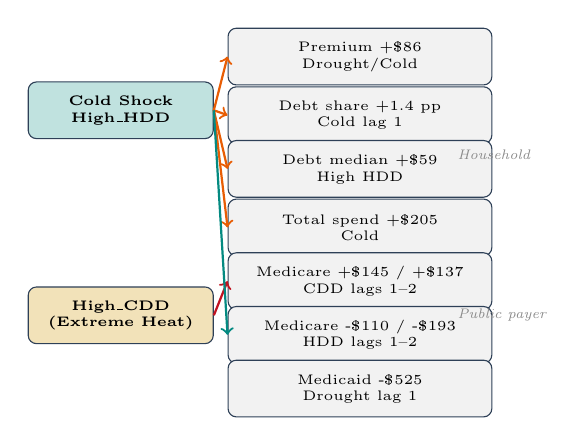
\begin{tikzpicture}[scale=0.62,
        box/.style={draw=DeepNavy, rounded corners=3pt, fill=LightGray,
                    minimum width=3.35cm, minimum height=0.72cm,
                    align=center, font=\tiny},
        cause/.style={draw=DeepNavy, rounded corners=3pt,
                    minimum width=2.35cm, minimum height=0.72cm,
                    align=center, font=\tiny\bfseries}]

        \node[cause, fill=Teal!25]  (cold) at (0, 0)    {Cold Shock\\High\_HDD};
        \node[cause, fill=Gold!30]  (heat) at (0,-4.2)  {High\_CDD\\(Extreme Heat)};

        \node[box] (prem)  at (4.9, 1.1)  {Premium +\$86\\Drought/Cold};
        \node[box] (dshare) at (4.9,-0.1) {Debt share +1.4 pp\\Cold lag 1};
        \node[box] (dmed)  at (4.9,-1.2)  {Debt median +\$59\\High HDD};
        \node[box] (exp)   at (4.9,-2.4)  {Total spend +\$205\\Cold};

        \node[box] (mc1)   at (4.9,-3.5)  {Medicare +\$145 / +\$137\\CDD lags 1--2};
        \node[box] (mc2)   at (4.9,-4.6)  {Medicare -\$110 / -\$193\\HDD lags 1--2};
        \node[box] (mcd)   at (4.9,-5.7)  {Medicaid -\$525\\Drought lag 1};

        \draw[->, WarmOrange, thick] (cold.east) -- (prem.west);
        \draw[->, WarmOrange, thick] (cold.east) -- (dshare.west);
        \draw[->, WarmOrange, thick] (cold.east) -- (dmed.west);
        \draw[->, WarmOrange, thick] (cold.east) -- (exp.west);
        \draw[->, DeepRed,    thick] (heat.east) -- (mc1.west);
        \draw[->, Teal,       thick] (cold.east) -- (mc2.west);

        \node[font=\tiny\itshape, text=WarmGray, anchor=west] at (6.7,-0.9) {Household};
        \node[font=\tiny\itshape, text=WarmGray, anchor=west] at (6.7,-4.2) {Public payer};
      \end{tikzpicture}
      \end{center}
    \end{column}
    \begin{column}{0.41\textwidth}
      \footnotesize
      \textbf{Cold channel:}
      \begin{itemize}\itemsep0.10em
        \item Premiums, debt, and total spending rise
        \item Medicare falls with lagged HDD exposure
      \end{itemize}
      \vspace{0.15em}
      \textbf{Heat channel (CDD):}
      \begin{itemize}\itemsep0.10em
        \item Medicare rises 1--2 years later
      \end{itemize}
      \vspace{0.15em}
      \textbf{Drought:}
      \begin{itemize}\itemsep0.10em
        \item Medicaid falls and premiums rise
      \end{itemize}
      \vspace{0.15em}
      \tealtext{\footnotesize Heat and cold affect public payers in\\opposite directions --- novel finding.}
    \end{column}
  \end{columns}
\end{frame}

% ── Slide 6 — State headline coefficients
\begin{frame}{State: Headline Coefficients}
  \framesubtitle{Selected significant lags; \(^{*}p{<}0.10\), \(^{**}p{<}0.05\), \(^{***}p{<}0.01\)}
  \scriptsize
  \begin{columns}[T]
    \begin{column}{0.50\textwidth}
      \tealtext{\textbf{Household outcomes}}\\[0.25em]
      \begin{tabular}{@{}>{\raggedright\arraybackslash}p{0.55\linewidth}rr@{}}
        \toprule
        Coefficient (state-clustered) & Estimate & \\
        \midrule
        Employer Prem.: Severe Drought ($h{=}0$) & $+\$86.4$  & \emphcolor{***} \\
        Employer Prem.: Severe Drought (lag 1)   & $+\$65.1$  & \emphcolor{**}  \\
        Employer Prem.: Pct PM$_{2.5}$ days      & $+\$20.8$  & \emphcolor{***} \\
        Debt Share: Cold Shock (lag 1)           & $+0.0135$  & \emphcolor{**}  \\
        Debt Median: High HDD ($h{=}0$)          & $+\$58.9$  & \emphcolor{**}  \\
        Debt Median: Heat Shock (lag 2)          & $+\$47.7$  & \emphcolor{**}  \\
        Total PC Health Exp: Cold Shock ($h{=}0$) & $+\$205.3$ & \emphcolor{**}  \\
        \bottomrule
      \end{tabular}
    \end{column}
    \begin{column}{0.46\textwidth}
      \tealtext{\textbf{Public payer outcomes}}\\[0.25em]
      \begin{tabular}{@{}>{\raggedright\arraybackslash}p{0.55\linewidth}rr@{}}
        \toprule
        Coefficient (state-clustered) & Estimate & \\
        \midrule
        Medicaid PE: Extreme Drought ($h{=}0$) & $-\$566.2$ & \emphcolor{**}  \\
        Medicaid PE: Severe Drought (lag 1)    & $-\$524.5$ & \emphcolor{***} \\
        Medicare PE: Severe Drought (lag 1)    & $-\$144.3$ & \emphcolor{***} \\
        Medicare PE: High CDD (lag 1)          & $+\$144.7$ & \emphcolor{**}  \\
        Medicare PE: High CDD (lag 2)          & $+\$137.2$ & \emphcolor{***} \\
        Medicare PE: High HDD (lag 1)          & $-\$110.1$ & \emphcolor{*}   \\
        Medicare PE: High HDD (lag 2)          & $-\$192.7$ & \emphcolor{***} \\
        \bottomrule
      \end{tabular}
    \end{column}
  \end{columns}
  \vspace{0.25em}
  \begin{center}
    \scriptsize \tealtext{Headline:} Extreme Drought lag-2 and Cold Shock lag-1 raise medical debt \& premiums; drought depresses Medicaid; heat and cold move Medicare in opposite directions.
  \end{center}
\end{frame}

% ━━━━━━━━━━━━━━━━━━━━━━━━━━━━━━━━━━━━━━━━━━━━━━━━━━━━━━━━━━━━━━━━━━━━━━━━━━━
% COUNTY-LEVEL RECAP
% ━━━━━━━━━━━━━━━━━━━━━━━━━━━━━━━━━━━━━━━━━━━━━━━━━━━━━━━━━━━━━━━━━━━━━━━━━━━
\transitionslide{County-Level Findings}{Cold raises debt and premiums; heat depresses income;\\hospital bad debt rises with cold and lagged drought}

% ── Slide 7 — County channel diagram
\begin{frame}{County-Level: Channels Mirror the State Findings}
  \begin{columns}[T]
    \begin{column}{0.58\textwidth}
      \vspace{0.2em}
      \begin{center}
      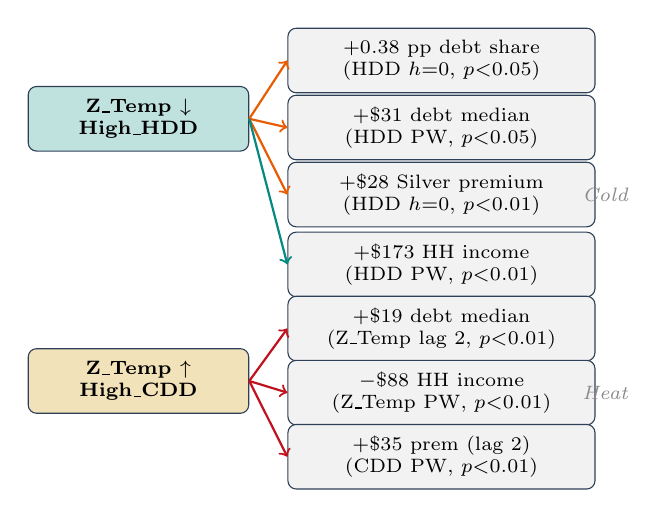
\begin{tikzpicture}[scale=0.74,
        box/.style={draw=DeepNavy, rounded corners=3pt, fill=LightGray,
                    minimum width=3.9cm, minimum height=0.82cm,
                    align=center, font=\scriptsize},
        cause/.style={draw=DeepNavy, rounded corners=3pt,
                    minimum width=2.8cm, minimum height=0.82cm,
                    align=center, font=\scriptsize\bfseries}]

        \node[cause, fill=Teal!25]  (cold) at (0, 0)    {Z\_Temp $\downarrow$\\High\_HDD};
        \node[cause, fill=Gold!30]  (heat) at (0,-4.5)  {Z\_Temp $\uparrow$\\High\_CDD};

        \node[box] (dshare) at (5.2, 1.0)  {$+0.38$ pp debt share\\(HDD $h{=}0$, $p{<}0.05$)};
        \node[box] (dmed)   at (5.2,-0.15) {$+\$31$ debt median\\(HDD PW, $p{<}0.05$)};
        \node[box] (prem)   at (5.2,-1.3)  {$+\$28$ Silver premium\\(HDD $h{=}0$, $p{<}0.01$)};
        \node[box] (hinc)   at (5.2,-2.5)  {$+\$173$ HH income\\(HDD PW, $p{<}0.01$)};

        \node[box] (dmed2)  at (5.2,-3.6)  {$+\$19$ debt median\\(Z\_Temp lag 2, $p{<}0.01$)};
        \node[box] (hinc2)  at (5.2,-4.7)  {$-\$88$ HH income\\(Z\_Temp PW, $p{<}0.01$)};
        \node[box] (prem2)  at (5.2,-5.8)  {$+\$35$ prem (lag 2)\\(CDD PW, $p{<}0.01$)};

        \draw[->, WarmOrange, thick] (cold.east) -- (dshare.west);
        \draw[->, WarmOrange, thick] (cold.east) -- (dmed.west);
        \draw[->, WarmOrange, thick] (cold.east) -- (prem.west);
        \draw[->, Teal,       thick] (cold.east) -- (hinc.west);
        \draw[->, DeepRed,    thick] (heat.east) -- (dmed2.west);
        \draw[->, DeepRed,    thick] (heat.east) -- (hinc2.west);
        \draw[->, DeepRed,    thick] (heat.east) -- (prem2.west);

        \node[font=\scriptsize\itshape, text=WarmGray, anchor=west] at (7.45,-1.3) {Cold};
        \node[font=\scriptsize\itshape, text=WarmGray, anchor=west] at (7.45,-4.7) {Heat};
      \end{tikzpicture}
      \end{center}
    \end{column}
    \begin{column}{0.38\textwidth}
      \scriptsize
      \textbf{Cold channel:}
      \begin{itemize}\itemsep0.05em
        \item Raises debt prevalence \& severity
        \item Raises premiums on impact
        \item \tealtext{Raises} HH income (energy mix)
      \end{itemize}
      \vspace{0.1em}
      \textbf{Heat channel:}
      \begin{itemize}\itemsep0.05em
        \item Raises debt median (lagged)
        \item \emphcolor{Reduces} HH income contemporaneously
        \item Raises premiums with 1--2 yr lag
      \end{itemize}
      \vspace{0.1em}
      \textbf{Cross-level alignment:}
      \begin{itemize}\itemsep0.05em
        \item Cold $\to$ debt: both levels confirm
        \item Heat $\to$ income: county only
        \item Premium channels align in direction
      \end{itemize}
    \end{column}
  \end{columns}
\end{frame}

% ── Slide 8 — County headline coefficients
\begin{frame}{County: Headline Coefficients and Hospital Channel}
  \framesubtitle{Two-way FE (fips + Year); state-clustered (RA-cluster for premiums); \emphcolor{**}\(p{<}0.05\), \emphcolor{***}\(p{<}0.01\)}
  \scriptsize
  \begin{columns}[T]
    \begin{column}{0.50\textwidth}
      \tealtext{\textbf{Premiums, debt, income (PW)}}\\[0.25em]
      \begin{tabular}{@{}>{\raggedright\arraybackslash}p{0.55\linewidth}rr@{}}
        \toprule
        Coefficient & Estimate & \\
        \midrule
        Benchmark Silver: High HDD ($h{=}0$) & $+\$21.9$ & \emphcolor{***} \\
        Benchmark Silver: High CDD (lag 2)   & $+\$35.3$ & \emphcolor{***} \\
        Debt Median (PW): High HDD ($h{=}0$) & $+\$31.2$ & \emphcolor{**}  \\
        Med HH Income: Z\_Temp ($h{=}0$)     & $-\$88$   & \emphcolor{***} \\
        Med HH Income: High HDD ($h{=}0$)    & $+\$173$  & \emphcolor{***} \\
        PCPI: PDSI lag 2                     & $-\$113$  & \emphcolor{**}  \\
        PCPI: RA-spec PDSI ($h{=}0$)         & $-\$206$  & \emphcolor{***} \\
        \bottomrule
      \end{tabular}
    \end{column}
    \begin{column}{0.46\textwidth}
      \tealtext{\textbf{Hospital bad debt per capita}}\\[0.25em]
      \begin{tabular}{@{}>{\raggedright\arraybackslash}p{0.55\linewidth}rr@{}}
        \toprule
        Coefficient & Estimate & \\
        \midrule
        High HDD ($h{=}0$)        & $+\$5.33$  & \emphcolor{***} \\
        Z\_Temp lag 2 (UW)        & $-\$2.41$  & \emphcolor{***} \\
        Z\_Temp lag 2 (PW)        & $-\$2.08$  & \emphcolor{***} \\
        PDSI lag 2 (PW)           & $+\$0.50$  & \emphcolor{*}   \\
        Uninsured Rate (control)  & $+\$151$   & \emphcolor{***} \\
        \bottomrule
      \end{tabular}
      \vspace{0.35em}
      \graytext{\scriptsize Cold raises hospital bad debt on impact; heat lag \emph{reduces} it; uninsured rate dominates.}
    \end{column}
  \end{columns}
\end{frame}

% ━━━━━━━━━━━━━━━━━━━━━━━━━━━━━━━━━━━━━━━━━━━━━━━━━━━━━━━━━━━━━━━━━━━━━━━━━━━
% WEATHER SWING RECAP
% ━━━━━━━━━━━━━━━━━━━━━━━━━━━━━━━━━━━━━━━━━━━━━━━━━━━━━━━━━━━━━━━━━━━━━━━━━━━
\transitionslide{Weather-Swing (Delta) Analysis}{Year-over-year climate volatility as a new source of variation;\\new findings the level specs missed}

% ── Slide 9 — Delta key results
\begin{frame}{Weather Swings: AQI Ratchet, Drought-PCPI, Temp-Debt}
  \framesubtitle{\(\Delta\)FE primary spec; LP horizons \(h=0\ldots3\); \(^{*}p{<}0.10\), \(^{**}p{<}0.05\), \(^{***}p{<}0.01\)}
  \scriptsize
  \begin{columns}[T]
    \begin{column}{0.50\textwidth}
      \tealtext{\textbf{Selected swing coefficients}}\\[0.25em]
      \begin{tabular}{@{}>{\raggedright\arraybackslash}p{0.50\linewidth}rr@{}}
        \toprule
        Coefficient & Estimate & \\
        \midrule
        \(\Delta\)HDD \(\to\) Silver Prem ($h{=}0$)         & $+0.033$  & \emphcolor{***} \\
        HDD Onset \(\to\) Silver Prem                       & $+\$49.5$ & \emphcolor{**}  \\
        \(\Delta\)Z\_Temp \(\to\) Debt Median ($h{=}3$)     & $+\$29.7$ & \emphcolor{***} \\
        \(\Delta\)Max\_AQI \(\to\) Hosp Bad Debt ($h{=}0$)  & $+0.005$  & \emphcolor{**}  \\
        \(\Delta\)Max\_AQI \(\to\) Hosp Bad Debt ($h{=}3$)  & $+0.016$  & \emphcolor{***} \\
        \(\Delta\)Z\_Precip \(\to\) PCPI ($h{=}1$)          & $-\$274$  & \emphcolor{***} \\
        \(\Delta\)PDSI     \(\to\) PCPI ($h{=}1$)           & $-\$226$  & \emphcolor{***} \\
        \bottomrule
      \end{tabular}
    \end{column}
    \begin{column}{0.46\textwidth}
      \textbf{\tealtext{What the delta analysis adds}}
      \begin{itemize}\itemsep0.16em
        \item \emphcolor{AQI ratchet} (h=3 effect 3\(\times\) h=0) --- level specs were null; volatility identifies cost
        \item \emphcolor{Drought worsening} drives PCPI loss; recovery asymmetrically weaker
        \item \emphcolor{Temp swing} accumulates into medical debt over 3 years
        \item \emphcolor{HDD onset pricing}: first-year cold raises Silver Premium \(\sim\)\$49
      \end{itemize}
      \vspace{0.25em}
      \graytext{\scriptsize \textbf{Key insight:} weather \emph{volatility} carries independent health-finance costs beyond level effects.}
    \end{column}
  \end{columns}
\end{frame}

% ━━━━━━━━━━━━━━━━━━━━━━━━━━━━━━━━━━━━━━━━━━━━━━━━━━━━━━━━━━━━━━━━━━━━━━━━━━━
% Cross-level synthesis
% ━━━━━━━━━━━━━━━━━━━━━━━━━━━━━━━━━━━━━━━━━━━━━━━━━━━━━━━━━━━━━━━━━━━━━━━━━━━
\begin{frame}{Cross-Level Synthesis}
  \framesubtitle{State, county, and weather-swing analyses tell a consistent story}
  \begin{center}
  \small
  \renewcommand{\arraystretch}{1.5}
  \begin{tabular}{lccc}
    \rowcolor{DeepNavy}
    \textcolor{white}{\textbf{Finding}} &
    \textcolor{white}{\textbf{State}} &
    \textcolor{white}{\textbf{County}} &
    \textcolor{white}{\textbf{Swing}} \\
    \rowcolor{Teal!10}
    Cold / HDD \(\to\) medical debt \(\uparrow\) &
    \tealtext{\textbf{\checkmark}} & \tealtext{\textbf{\checkmark}} & \tealtext{\textbf{\checkmark}} \\
    Cold / HDD \(\to\) premiums \(\uparrow\) &
    \tealtext{\textbf{\checkmark}} & \tealtext{\textbf{\checkmark}} & \tealtext{\textbf{\checkmark}} \\
    \rowcolor{Teal!10}
    Cold / HDD \(\to\) hospital bad debt \(\uparrow\) &
    \graytext{---} & \tealtext{\textbf{\checkmark}} & \graytext{---} \\
    Drought \(\to\) Medicaid \(\downarrow\) / PCPI \(\downarrow\) &
    \tealtext{\textbf{\checkmark}} & \tealtext{\textbf{\checkmark}} & \tealtext{\textbf{\checkmark}} \\
    \rowcolor{Teal!10}
    Heat / CDD \(\to\) HH income \(\downarrow\) (lag) &
    \graytext{---} & \tealtext{\textbf{\checkmark}} & \graytext{(asym.)} \\
    AQI \(\to\) hospital bad debt \(\uparrow\) &
    \graytext{(weak)} & \graytext{(weak)} & \tealtext{\textbf{\checkmark} (new)} \\
    \rowcolor{Teal!10}
    Heat vs.\ cold on \emph{Medicare} (opposite signs) &
    \tealtext{\textbf{\checkmark}} & \graytext{(partial)} & \graytext{---} \\
  \end{tabular}
  \end{center}
  \vspace{0.4em}
  \begin{center}
  \footnotesize \tealtext{Headline:} cold shocks raise household financial burden;
  drought hits public payers and PCPI;
  weather \emph{volatility} adds an independent channel (AQI ratchet; temp-debt accumulation).
  \end{center}
\end{frame}

% ━━━━━━━━━━━━━━━━━━━━━━━━━━━━━━━━━━━━━━━━━━━━━━━━━━━━━━━━━━━━━━━━━━━━━━━━━━━
% PART 2 — Committee Feedback Response
% ━━━━━━━━━━━━━━━━━━━━━━━━━━━━━━━━━━━━━━━━━━━━━━━━━━━━━━━━━━━━━━━━━━━━━━━━━━━
\transitionslide{Part 2 --- Committee Feedback Response}{Random effects, post-exit dynamics, never-exposed DiD,\\propagation evidence, humidity (April 2026 review)}

% ── What the committee asked
\begin{frame}{What the Committee Asked}
  \framesubtitle{Five concerns across three domains, all addressed in this update except humidity}
  \begin{columns}[T]
    \begin{column}{0.47\textwidth}
      \textbf{\tealtext{Econometric}}
      \begin{itemize}\itemsep0.15em
        \item \emphcolor{Check random effects} as an alternative to FE
        \item \emphcolor{Lag / exit tests}: what happens when a county leaves a shock state?
        \item Find \emphcolor{natural experiments} for DiD --- are there never-exposed counties?
      \end{itemize}
      \vspace{0.4em}
      \textbf{\tealtext{General}}
      \begin{itemize}\itemsep0.15em
        \item \emphcolor{Propagation pathways} must be backed by evidence (heat \(\to\) delayed care; cold \(\to\) utilization shifts)
      \end{itemize}
    \end{column}
    \begin{column}{0.47\textwidth}
      \textbf{\tealtext{Environmental}}
      \begin{itemize}\itemsep0.15em
        \item Add \emphcolor{humidity} (PRISM \texttt{tdmean}) at state level
      \end{itemize}
      \vspace{0.5em}
      \textbf{\tealtext{Response status}}\\[0.2em]
      \footnotesize
      \begin{tabular}{@{}>{\raggedright\arraybackslash}p{0.55\linewidth}>{\raggedright\arraybackslash}p{0.32\linewidth}@{}}
        \toprule
        Concern & Status \\
        \midrule
        Random effects & Done \\
        Post-exit dynamics & Done \\
        Never-exposed DiD & Done \\
        Propagation pathways & Done \\
        Humidity (PRISM) & \emphcolor{Parked} \\
        \bottomrule
      \end{tabular}
    \end{column}
  \end{columns}
\end{frame}

% ── RE robustness
\begin{frame}{Random Effects Is Rejected; Headlines Survive}
  \framesubtitle{Hausman tests on primary FE specs; matched plm two-way effects}
  \begin{columns}[T]
    \begin{column}{0.50\textwidth}
      \textbf{\tealtext{Design}}
      \begin{itemize}\itemsep0.12em
        \item Two-way FE vs.\ RE GLS on the same RHS; Hausman test per outcome
        \item 11 outcomes estimable (4 state, 7 county)
      \end{itemize}
      \vspace{0.25em}
      \textbf{\tealtext{Verdict}}
      \begin{itemize}\itemsep0.12em
        \item \emphcolor{RE rejected for every estimable outcome at \(p<10^{-9}\)}
        \item Headlines (Drought lag-2, Cold lag-1) have the \emphcolor{same sign} in RE
        \item Only Medicaid Per Enrollee shows material FE/RE divergence (\(\sim\)2\(\times\))
      \end{itemize}
    \end{column}
    \begin{column}{0.46\textwidth}
      \textbf{\tealtext{Selected Hausman results}}\\[0.25em]
      \scriptsize
      \begin{tabular}{@{}>{\raggedright\arraybackslash}p{0.45\linewidth}rr@{}}
        \toprule
        Outcome & \(\chi^2\) & \(p\)-value \\
        \midrule
        \multicolumn{3}{l}{\textit{State}} \\
        Medical Debt Share          & 233.6 & 4.5e-40 \\
        Total PC Health Exp         & 247.9 & 5.7e-43 \\
        Medicaid PE Health Exp      & 81.3  & 2.3e-10 \\
        Medicare PE Health Exp      & 834.4 & 2.1e-166 \\
        \midrule
        \multicolumn{3}{l}{\textit{County}} \\
        Medical Debt Share          & 23{,}905 & $<$1e-300 \\
        Benchmark Silver Real       & 23{,}545 & $<$1e-300 \\
        PCPI Real                   & 5{,}809  & $<$1e-300 \\
        Civilian Employed           & 220.2 & 4.6e-41 \\
        \bottomrule
      \end{tabular}
    \end{column}
  \end{columns}
\end{frame}

% ── Post-exit dynamics
\begin{frame}{Post-Exit Dynamics --- What Happens When a County Leaves Shock State?}
  \framesubtitle{Local projections of \(*\_\text{Exit}\) at \(h=0,1,2,3\); answers the committee's exit-test question directly}
  \begin{columns}[T]
    \begin{column}{0.31\textwidth}
      \textbf{\tealtext{Drought\_Exit}}
      \begin{itemize}\itemsep0.12em
        \item \emphcolor{PCPI partial scarring}: \(+\$1{,}044\) p.c.\ at \(h=2\) (\(p=0.0002\))
        \item Recovery rebounds but does not fully restore pre-shock income
        \item Confirmed by Block B interaction (\(+\$964\) at \(h=2\), \(p=0.010\))
      \end{itemize}
    \end{column}
    \begin{column}{0.31\textwidth}
      \textbf{\tealtext{HDD\_Exit}}
      \begin{itemize}\itemsep0.12em
        \item \emphcolor{Immediate hospital-cost relief}: \(-3.13\) p.c.\ at \(h=0\) (\(p=0.014\))
        \item Sustained at \(h=2\): \(-2.88\) (\(p=0.034\))
        \item Cold-shock cost is in the \emphcolor{exposure}, not lasting damage
      \end{itemize}
    \end{column}
    \begin{column}{0.31\textwidth}
      \textbf{\tealtext{CDD\_Exit}}
      \begin{itemize}\itemsep0.12em
        \item Persistent employment benefits after exit
        \item Likely part secular regional trend (caveated)
        \item Phase 2 LP rejects within-county heat scarring
      \end{itemize}
    \end{column}
  \end{columns}
\end{frame}

% ── Post-Exit LP visuals
\begin{frame}{Post-Exit LP: Shock-Specific Recovery Patterns}
  \framesubtitle{Drought partially scars income; cold-shock exit brings immediate hospital-cost relief}
  \begin{columns}[T]
    \begin{column}{0.48\textwidth}
      \begin{center}
        \textbf{\tealtext{\small Drought\_Exit \(\to\) PCPI Real}}\\[0.1em]
        \includegraphics[width=\textwidth, height=0.50\textheight, keepaspectratio]%
          {../Analysis/plots/delta_exit_dynamics/exit_lp_Drought_Exit_PCPI_Real.png}
      \end{center}
      \vspace{-0.4em}
      \graytext{\scriptsize Peak at \(h=2\): \(+\$1{,}044\) (\(p=0.0002\)). Partial recovery.}
    \end{column}
    \begin{column}{0.48\textwidth}
      \begin{center}
        \textbf{\tealtext{\small HDD\_Exit \(\to\) Hosp.\ Bad Debt / Capita}}\\[0.1em]
        \includegraphics[width=\textwidth, height=0.50\textheight, keepaspectratio]%
          {../Analysis/plots/delta_exit_dynamics/exit_lp_HDD_Exit_Hosp_BadDebt_PerCapita.png}
      \end{center}
      \vspace{-0.4em}
      \graytext{\scriptsize Relief at \(h=0\) (\(-3.13\), \(p=0.014\)); sustained at \(h=2\). No scarring.}
    \end{column}
  \end{columns}
\end{frame}

% ── Phase 0 inventory
\begin{frame}{Phase 0: Are There Never-Exposed Counties?}
  \framesubtitle{Inventory of zero-event counties over 2011--2023; feasibility memo selected primary cohorts}
  \begin{columns}[T]
    \begin{column}{0.52\textwidth}
      \textbf{\tealtext{Never-exposed pool by shock}}\\[0.25em]
      \scriptsize
      \begin{tabular}{@{}>{\raggedright\arraybackslash}p{0.50\linewidth}rrr@{}}
        \toprule
        Shock & Total & Never-exposed & Share \\
        \midrule
        Extreme Drought (PDSI \(\le -4\))    & 3{,}225 & \textbf{2{,}534} & 78.6\% \\
        High HDD (top quintile)              & 3{,}225 & \textbf{2{,}303} & 71.4\% \\
        High CDD (top quintile)              & 3{,}225 & \textbf{2{,}121} & 65.8\% \\
        High AQI Max ($>$100)                & 3{,}225 & 100              & \emphcolor{3.1\%} \\
        \bottomrule
      \end{tabular}
      \vspace{0.45em}
      \begin{itemize}\itemsep0.15em
        \item Drought, HDD, CDD all have large never-exposed pools
        \item \emphcolor{AQI dropped from DiD}: 3.1\% control pool too thin
      \end{itemize}
    \end{column}
    \begin{column}{0.42\textwidth}
      \textbf{\tealtext{Candidate sharp events}}\\[0.25em]
      \scriptsize
      \begin{tabular}{@{}>{\raggedright\arraybackslash}p{0.50\linewidth}rr@{}}
        \toprule
        Event & Onsets & Onset rate \\
        \midrule
        \emphcolor{2012 Midwest Drought} & 139 & 4.4\% \\
        2022 Drought                     & 110 & 3.5\% \\
        \emphcolor{2013 HDD (cold)}      & 407 & 13.0\% \\
        2018 CDD (heat)                  & 250 & 8.0\% \\
        2023 AQI (wildfire smoke)        & 336 & 34.1\% \\
        \bottomrule
      \end{tabular}
    \end{column}
  \end{columns}
\end{frame}

% ── 2012 Drought 2x2
\begin{frame}{2012 Midwest Drought: The Cleanest Natural Experiment}
  \framesubtitle{139 first-event counties (treatment) vs.\ 2{,}534 never-exposed (control), 2011--2023}
  \begin{columns}[T]
    \begin{column}{0.50\textwidth}
      \textbf{\tealtext{Design}}\\[0.2em]
      \footnotesize
      \(Y_{it} = \alpha_i + \gamma_t + \tau\,(\text{Treated}_i \times \text{Post}_t) + \varepsilon_{it}\)
      \begin{itemize}\itemsep0.15em
        \item Treated: first-ever Extreme Drought event \(=\) 2012
        \item Control: never experienced Extreme Drought in panel window
        \item Cluster: state; SE: \texttt{feols(\(\ldots\), cluster="State")}
      \end{itemize}
      \vspace{0.3em}
      \textbf{\tealtext{Why this is the cleanest piece}}
      \begin{itemize}\itemsep0.10em
        \item Within-county LP cannot rule out recurring-shock confounding
        \item 2x2 against never-exposed \emphcolor{closes that loophole}
        \item 2012 drought is a documented event with defined geography
      \end{itemize}
    \end{column}
    \begin{column}{0.46\textwidth}
      \textbf{\tealtext{2x2 ATT results}}\\[0.25em]
      \footnotesize
      \begin{tabular}{@{}>{\raggedright\arraybackslash}p{0.48\linewidth}rr@{}}
        \toprule
        Outcome & ATT & \(p\) \\
        \midrule
        Medical Debt Share        & \(-0.0062\) & 0.49 \\
        Hosp Bad Debt PC          & \(+6.26\)   & 0.29 \\
        \emphcolor{PCPI Real}     & \emphcolor{\(-\$1{,}311\)} & \emphcolor{0.027} \\
        Med HH Income Real        & \(-\$992\)  & 0.24 \\
        \emphcolor{Civilian Employed} & \emphcolor{\(-2{,}053\)} & \emphcolor{0.0001} \\
        Benchmark Silver Real     & --- & ACA collinearity \\
        \bottomrule
      \end{tabular}
    \end{column}
  \end{columns}
\end{frame}

% ── 2012 Drought event study
\begin{frame}{2012 Drought DiD: Employment Loss Accumulates Over the Event Window}
  \framesubtitle{Event-study with leads/lags; reference \(t = -1\); cluster = State; treated vs.\ never-exposed only}
  \begin{columns}[T]
    \begin{column}{0.55\textwidth}
      \begin{center}
        \includegraphics[width=\textwidth, height=0.72\textheight, keepaspectratio]%
          {../Analysis/plots/did/eventstudy_Drought_2012_Civilian_Employed.png}
      \end{center}
    \end{column}
    \begin{column}{0.41\textwidth}
      \footnotesize
      \textbf{\tealtext{Reading the figure}}
      \begin{itemize}\itemsep0.15em
        \item \(t=0\): year of first drought event (2012)
        \item Visible \emphcolor{near-zero pre-period} at \(t=0\) (only 1 pre-year given panel start in 2011)
        \item Post-event employment loss \emphcolor{accumulates}: \(\sim\)-100 at \(t=1\); \(\sim\)-550 at \(t=2\); \(\sim\)-1{,}100 at \(t=3\)
        \item Consistent with the income-channel pathway feeding into employment
      \end{itemize}
      \vspace{0.3em}
      \graytext{\scriptsize Same identification, different outcome: PCPI Real follows the same downward profile (peak ATT \(-\$1{,}311\)).}
    \end{column}
  \end{columns}
\end{frame}

% ── CS-DiD
\begin{frame}{Callaway-Sant'Anna: Long-Run Cold-State Scarring}
  \framesubtitle{Cohort-weighted ATT(e) on HDD with never-treated controls; long-run damage compounds over a decade}
  \begin{columns}[T]
    \begin{column}{0.55\textwidth}
      \begin{center}
        \textbf{\tealtext{\small HDD \(\to\) Civilian\_Employed (CS-DiD)}}\\[0.15em]
        \includegraphics[width=\textwidth, height=0.62\textheight, keepaspectratio]%
          {../Analysis/plots/did/csdid_HDD_Civilian_Employed.png}
      \end{center}
      \vspace{-0.2em}
      \graytext{\scriptsize Cumulative loss grows from $\sim$0 at $e=0$ to \emphcolor{\(-4{,}982\) at \(e=10\)} (\(p=0.003\)). Medical Debt Share \(+4.9\)pp at $e=10$.}
    \end{column}
    \begin{column}{0.41\textwidth}
      \footnotesize
      \textbf{\tealtext{Drought (4 cohorts, 268 treated)}}
      \begin{itemize}\itemsep0.10em
        \item PCPI at \(e=0\): \emphcolor{\(-\$1{,}050\)} (\(p=0.002\))
        \item Civilian Employed at \(e=11\): \(-3{,}915\) (\(p=0.0001\))
      \end{itemize}
      \vspace{0.25em}
      \textbf{\tealtext{HDD (2 cohorts, 230 treated)}}
      \begin{itemize}\itemsep0.10em
        \item Long-run scarring in employment and debt-share
        \item Cumulative through \(e=6\)--10
      \end{itemize}
      \vspace{0.25em}
      \textbf{\tealtext{CDD: noisy, regional confounds}}
      \begin{itemize}\itemsep0.10em
        \item Treatment concentrated in TX/GA/MS/FL; controls in north
        \item Signs reverse across horizons --- \emphcolor{de-emphasize}
      \end{itemize}
    \end{column}
  \end{columns}
\end{frame}

% ── LP vs DiD reconciliation
\begin{frame}{LP and DiD Are Complementary, Not Contradictory}
  \framesubtitle{The cold-scarring puzzle resolves once we see both designs measure different things}
  \begin{columns}[T]
    \begin{column}{0.48\textwidth}
      \textbf{\tealtext{Local Projections / Exit-LP}}
      \begin{itemize}\itemsep0.15em
        \item Estimand: within-county response when shock state changes year-over-year
        \item HDD\_Exit \(\to\) hospital-cost relief at \(h=0\)
        \item \emphcolor{Read:} no within-county cold scarring after recovery
      \end{itemize}
    \end{column}
    \begin{column}{0.48\textwidth}
      \textbf{\tealtext{CS-DiD with never-exposed}}
      \begin{itemize}\itemsep0.15em
        \item Estimand: persistent gap between ever-treated and never-treated populations
        \item HDD long-run: \(-4{,}982\) jobs and \(+4.9\)pp debt share at \(e=10\)
        \item \emphcolor{Read:} treated counties end up worse off long-run
      \end{itemize}
    \end{column}
  \end{columns}
  \vspace{0.7em}
  \begin{center}
  \footnotesize
  \fbox{\parbox{0.92\textwidth}{\centering
    \textbf{\tealtext{Reconciliation:}} cold-shock counties \emph{recover} when shocks end (LP),
    but they \emph{spend more years in shock state} than never-exposed counties do,
    so the \emphcolor{population gap accumulates} (CS-DiD). Both are correct;
    they measure different things.}}
  \end{center}
\end{frame}

% ── Propagation pathways
\begin{frame}{Propagation Pathways --- Now Evidence-Backed}
  \framesubtitle{Each headline channel anchored to 2--4 peer-reviewed references with direction and time-scale}
  \scriptsize
  \begin{tabular}{@{}>{\raggedright\arraybackslash}p{0.20\linewidth}>{\raggedright\arraybackslash}p{0.27\linewidth}>{\raggedright\arraybackslash}p{0.32\linewidth}>{\raggedright\arraybackslash}p{0.14\linewidth}@{}}
    \toprule
    Pathway & Time-scale claim & Where identified & Strength \\
    \midrule
    Heat \(\to\) delayed care
      & Within-year deferral; lag-1/2 utilization
      & County Spec 2, CS-DiD CDD
      & Moderate \\
    Cold \(\to\) utilization shift
      & Contemporaneous + lag-1; long-run scarring at \(e\geq 8\)
      & State cold-shock lag-1, CS-DiD HDD
      & Strong \\
    Drought \(\to\) income \(\to\) debt
      & Lag-1, lag-2 income; debt follows
      & State drought lag-2, 2012 DiD, Exit-LP recovery
      & \emphcolor{Strongest} \\
    AQI \(\to\) respiratory / cardiac
      & Within-year, episodic spikes
      & County continuous AQI, event-study, swing analysis
      & Limited \\
    \bottomrule
  \end{tabular}
  \vspace{0.35em}
  \tiny
  \textbf{\tealtext{Refs}}\ \ \textbf{Drought:} Hornbeck (2012); Burke-Hsiang-Miguel (2015); Carleton et al.\ (2022).\ \
  \textbf{Cold:} Desch\^enes-Moretti (2009); Gasparrini et al.\ (2015); Andrews et al.\ (2017).\ \
  \textbf{Heat:} Sun et al.\ (2021); White (2017); Karlsson-Ziebarth (2018).\ \
  \textbf{AQI:} Deryugina et al.\ (2019); Schlenker-Walker (2016); Currie-Walker (2011).
\end{frame}

% ── Humidity parked
\begin{frame}{Humidity Integration --- Status and Resumption Plan}
  \framesubtitle{Phase 4 deferred; the highest-priority residual gap from committee feedback}
  \begin{columns}[T]
    \begin{column}{0.48\textwidth}
      \textbf{\tealtext{What we know}}
      \begin{itemize}\itemsep0.15em
        \item PRISM gridded endpoint returns monthly BIL rasters
        \item No state-aggregate API; must aggregate locally
        \item \(\sim\)408 monthly rasters, \(\sim\)1.5 GB on disk
      \end{itemize}
      \vspace{0.4em}
      \textbf{\tealtext{Blocker}}
      \begin{itemize}\itemsep0.15em
        \item Raster \(\to\) state polygon aggregation needs three R spatial packages
        \item Not installed in local R 4.2.2; Windows install pulls heavy system deps (GDAL/GEOS/PROJ)
      \end{itemize}
    \end{column}
    \begin{column}{0.48\textwidth}
      \textbf{\tealtext{Resumption plan}}
      \begin{itemize}\itemsep0.10em
        \item Install spatial stack; download monthly tdmean
        \item Aggregate to state-year; join into master
        \item Re-run; test \emphcolor{drought lag-2} and \emphcolor{cold lag-1} survival
      \end{itemize}
      \vspace{0.2em}
      \textbf{\tealtext{Why this matters}}
      \begin{itemize}\itemsep0.10em
        \item Single residual gap from committee feedback
        \item Low-humidity confounding remains open
      \end{itemize}
    \end{column}
  \end{columns}
\end{frame}

% ── What changed substantively
\begin{frame}{The Analysis Now Has Two Pieces of Stronger Identification}
  \framesubtitle{And one genuine puzzle resolved by treating LP and DiD as complementary}
  \begin{columns}[T]
    \begin{column}{0.48\textwidth}
      \textbf{\tealtext{New evidence}}
      \begin{itemize}\itemsep0.15em
        \item \emphcolor{2012 Drought 2x2} is now the cleanest single identification piece (PCPI \(-\$1{,}311\); Employed \(-2{,}053\))
        \item \emphcolor{HDD long-run scarring} (\(-4{,}982\) jobs at \(e=10\); \(+4.9\)pp debt share at \(e=10\)) was not visible in the within-county LP framework
        \item Drought\_Exit shows \emphcolor{partial income scarring} --- recovery rebounds but does not fully restore
      \end{itemize}
    \end{column}
    \begin{column}{0.48\textwidth}
      \textbf{\tealtext{Resolved puzzle}}
      \begin{itemize}\itemsep0.15em
        \item Cold counties \emphcolor{recover on exit} (no within-county scarring)
        \item But the ever-treated population \emphcolor{ends up worse off} long-run (DiD)
        \item Both findings are correct; they measure different things
      \end{itemize}
      \vspace{0.3em}
      \textbf{\tealtext{Methodological closure}}
      \begin{itemize}\itemsep0.15em
        \item Random effects rejected; FE is the right spec
        \item AQI exclusion from DiD now defensible (3.1\% never-exposed)
      \end{itemize}
    \end{column}
  \end{columns}
\end{frame}

% ── Open caveats
\begin{frame}{Open Caveats and Residual Risks}
  \framesubtitle{What the committee should know is still not addressed}
  \begin{columns}[T]
    \begin{column}{0.48\textwidth}
      \textbf{\tealtext{Humidity confounding}}
      \begin{itemize}\itemsep0.10em
        \item PRISM tdmean not yet a control
        \item Headline drought lag-2 and cold lag-1 \emphcolor{not stress-tested} against humidity
        \item Mitigation: resumption plan in place
      \end{itemize}
      \vspace{0.25em}
      \textbf{\tealtext{CDD CS-DiD region confound}}
      \begin{itemize}\itemsep0.10em
        \item Treatment concentrated south; controls north
        \item Two-way FE leaves regional trends
        \item Reported as \emphcolor{suggestive only}
      \end{itemize}
    \end{column}
    \begin{column}{0.48\textwidth}
      \textbf{\tealtext{Multiple testing}}
      \begin{itemize}\itemsep0.10em
        \item 427 ATT(g,t) cells \(\times\) 7 outcomes \(\times\) up to 11 event-times
        \item Headline cells survive Bonferroni within-shock
        \item Smaller-cohort cells do not
      \end{itemize}
      \vspace{0.25em}
      \textbf{\tealtext{County-master deduping}}
      \begin{itemize}\itemsep0.10em
        \item Master not strict one-row-per-(fips, year)
        \item Deduped in every analysis script
        \item Underlying fix deferred
      \end{itemize}
    \end{column}
  \end{columns}
\end{frame}

% ━━━━━━━━━━━━━━━━━━━━━━━━━━━━━━━━━━━━━━━━━━━━━━━━━━━━━━━━━━━━━━━━━━━━━━━━━━━
% Closing
% ━━━━━━━━━━━━━━━━━━━━━━━━━━━━━━━━━━━━━━━━━━━━━━━━━━━━━━━━━━━━━━━━━━━━━━━━━━━
\begingroup
\setbeamercolor{background canvas}{bg=DeepNavy}
\setbeamertemplate{footline}{}
\begin{frame}[plain]
  \begin{tikzpicture}[overlay]
    \node[text=Teal, opacity=0.12, font=\fontsize{140}{140}\selectfont]
      at (10, 2.5) {?};
  \end{tikzpicture}
  \vspace{2.4cm}
  \hspace{0.8cm}%
  {\color{white}\bfseries\fontsize{32}{36}\selectfont
    \parbox{13cm}{Thank you.}}
  \par\vspace{0.6em}
  \hspace{0.8cm}%
  {\color{WarmOrange}\rule{12cm}{2pt}}
  \par\vspace{0.6em}
  \hspace{0.8cm}%
  {\color{Teal}\Large Discussion and questions}
\end{frame}
\endgroup

\end{document}
